\documentclass[12pt]{article}
\usepackage[margin=1in]{geometry}
\usepackage[utf8]{inputenc}
\usepackage[spanish]{babel}
\usepackage{parskip}
\usepackage{setspace}
\usepackage{amsmath, amssymb}
\usepackage{tikz}
\usepackage{hyperref} % Siempre debe ir al final.

% Opciones de Paquetes.
\decimalpoint          % {babel}
\onehalfspacing        % {setspace}
\usetikzlibrary{babel} % {tikz}: Para que tikz no conflictue con {babel} con figuras como "->".
\graphicspath{{./img/}} % {graphics}: Indica ruta de donde se importan las imágenes.

\title{Clase 2. Determinantes y el Producto Cruz.}
\author{MIT 18.02: Multivariable Calculus.}
\date{}


\begin{document}

% Comandos personalizados.
%=========================================
%
%    Comandos personalizados usados en
%       los apuntes de este curso.
%
%=========================================

\newcommand{\vecmat}[1]{\mathbf{#1}}                          % Vectores o matrices en negrita en math mode.
\newcommand{\unitvec}[1]{\vecmat{\hat{#1}}}                   % Vectores unitarios.
\newcommand{\overvec}[1]{\overrightarrow{#1}}                 % Vector como segmento orientado.
\newcommand{\proy}[2]{\text{proy}_{\vecmat{#2}}{\vecmat{#1}}} % Proyección vectorial.
\newcommand{\invmat}[1]{\vecmat{#1}^{-1}}                     % Inversa de una matriz.
\newcommand{\transmat}[1]{\vecmat{#1}^{T}}                    % Transpuesta de una matriz.
\newcommand{\Adj}[0]{\text{Adj}}                              % Matriz adjunta.
\newcommand{\R}[0]{\mathbb{R}}                                % Símbolo conjunto de los números reales.
\newcommand{\N}[0]{\mathbb{N}}                                % Símbolo conjunto de los números naturales.


\maketitle

\begin{abstract}
\noindent En esta clase se estudiará preliminarmente al escalar llamado \textbf{determinante}. El enfoque estará en su interpretación geométrica. Luego se verá otra operación relevante entre vectores que recibe el nombre de \textbf{producto cruz}.
\end{abstract}


\section{Determinantes.}

El \textbf{determinante} es un \textbf{escalar} calculado mayormente en matrices, ya que entrega información relevante de éstas\footnote{Lo veremos en la siguiente clase.}. A nivel geométrico, equivale a los valores absolutos del área de un paralelogramo y del volumen de un paralelepipedo. Ambos pueden obtenerse usando vectores.

En general, solo es posible calcular el determinante de una \textbf{cantidad de vectores que es igual a su dimensión}. Acá nos concentraremos solo en aquellos de dos y tres dimensiones.

Sean dos vectores $\vecmat{a}, \ \vecmat{b} \in \R^{2}$. El determinante de ambos se calcula como:
\[
\det(\vecmat{a}, \ \vecmat{b}) =
\begin{vmatrix}
a_{1} & a_{2} \\
b_{1} & b_{2}
\end{vmatrix} =
a_{1}b_{2} - a_{2}b_{1}
\]
Por otra parte, si $\vecmat{a}, \ \vecmat{b}, \ \vecmat{c} \in \R^{3}$, el determinante entre todos ellos se puede obtener como:
\begin{align*}
\det(\vecmat{a}, \ \vecmat{b}, \ \vecmat{c}) &=
\begin{vmatrix}
a_{1} & a_{2} & a_{3} \\
b_{1} & b_{2} & b_{3} \\
c_{1} & c_{2} & c_{3}
\end{vmatrix}
= a_{1} \ 
\begin{vmatrix}
b_{2} & b_{3} \\
c_{2} & c_{3}
\end{vmatrix}
- a_{2} \ 
\begin{vmatrix}
b_{1} & b_{3} \\
c_{1} & c_{3}
\end{vmatrix}
+ a_{3} \ 
\begin{vmatrix}
b_{1} & b_{2} \\
c_{1} & c_{2}
\end{vmatrix} \\
&= (b_{2}c_{3} - b_{3}c_{2}) a_{1} - (b_{1}c_{3} - b_{3}c_{1}) a_{2} + (b_{1}c_{2} - b_{2}c_{1}) a_{3}
\end{align*}
El método usado para calcular $\det(\vecmat{a}, \ \vecmat{b}, \ \vecmat{c})$ se conoce como ``expansión por la primera fila'' del determinante.

Veamos cómo el determinante de dos vectores se iguala al área de un paralelogramo.

\subsection{Área de un paralelogramo.}

Considere dos vectores de posición $\vecmat{a}, \ \vecmat{b} \in \R^{2}$. Al unirlos en sus puntos iniciales, es posible formar un paralelogramo de altura $h$ como se observa en la siguiente figura.

\begin{figure}[hbt!]
\centering

\begin{tikzpicture}
% Líneas de ayuda.
%\draw[color = lightgray] (0, 0) grid (13, 5);

% Ejes de coordenadas.
\draw[-latex, line width = 0.3mm, color = black!80] (5, 0.6) -- (5, 4.5) node[left, color = black] {$y$};
\draw[-latex, line width = 0.3mm, color = black!80] (4.6, 1) -- (9, 1) node[below, color = black] {$x$};
\node at (4.8, 0.75) {$0$};

% Área del paralelogramo.
\draw[fill = gray!50, color = gray!20] (5, 1) -- (9, 2.3) -- (10.2, 4.8) -- (7, 4) -- (5, 1);

%Lados del paralelogramo.
\draw[style = dashed, line width = 0.3mm, color = gray] (9, 2.3) -- (10.2, 4.8) -- (7, 4) -- node[right, color = black] {$h$} (7.65, 1.77);
\draw[color = gray, fill = gray] (7.65, 1.85) -- (7.57, 2.1) -- (7.34, 2.03) -- (7.42, 1.77) -- cycle;
\node at (9, 3.7) {$A_{p}$};

% Vectores.
\draw[-stealth, line width = 0.5mm] (5, 1) -- node[below right] {$\vecmat{a}$} (9, 2.3); % a
\draw[-stealth, line width = 0.5mm] (5, 1) -- node[above left] {$\vecmat{b}$} (7, 4);    % b
\node at (5.7, 1.5) {$\theta$};
\end{tikzpicture}

\end{figure}

Con la información que está en la figura busquemos el área del paralelogramo, $A_{p}$.

Formalmente, $A_{p}$ se calcula como:
\[
  A_{p} = \text{base} \cdot \text{altura} = ||\vecmat{a}|| \cdot h
\]
Mediante la figura del paralelogramo, se puede calcular su altura como:
\begin{align*}
  \sin(\theta) &= \frac{h}{||\vecmat{b}||} \\
  \therefore h &= ||\vecmat{b}|| \cdot \sin(\theta)
\end{align*}
Al reemplazar a $h$ en $A_{p}$:
\[
  A_{p} = ||\vecmat{a}|| \cdot ||\vecmat{b}|| \cdot \sin(\theta)
\]
La fórmula de $A_{p}$ es similar a la de $\vecmat{a} \cdot \vecmat{b}$. La llevaremos a esta operación porque permitirá depender solo de los componentes de estos vectores, sin necesidad de conocer a $\theta$.

Sea $\vecmat{a}'$ el vector $\vecmat{a}$ rotado en $\frac{\pi}{2}$ radianes. Esto implica que $||\vecmat{a}|| = ||\vecmat{a}'||$, pero $\vecmat{a}' = \langle -a_{2}, \ a_{1} \rangle$.

\newpage

\begin{figure}[hbt!]
\centering

\begin{tikzpicture}
% Líneas de ayuda.
%\draw[color = lightgray] (0, 0) grid (13, 5);

% Ejes de coordenadas.
\draw[-latex, line width = 0.3mm, color = black!80] (5, 0.6) -- (5, 4.5) node[left, color = black] {$y$};
\draw[-latex, line width = 0.3mm, color = black!80] (4.6, 1) -- (9, 1) node[below, color = black] {$x$};
\node at (4.8, 0.75) {$0$};

% Área del paralelogramo.
\draw[fill = gray!50, color = gray!20] (5, 1) -- (9, 2.3) -- (10.2, 4.8) -- (7, 4) -- (5, 1);

%Lados del paralelogramo.
\draw[style = dashed, line width = 0.3mm, color = gray] (9, 2.3) -- (10.2, 4.8) -- (7, 4) -- node[right, color = black] {$h$} (7.65, 1.77);
\draw[color = gray, fill = gray] (7.65, 1.85) -- (7.57, 2.1) -- (7.34, 2.03) -- (7.42, 1.77) -- cycle;
\node at (9, 3.7) {$A_{p}$};

% Vectores.
\draw[color = gray, fill = gray] (5.36, 1.09) -- (5.208, 1.45) -- (4.9, 1.32) -- (5, 1) -- cycle;
\draw[-stealth, line width = 0.5mm] (5, 1) -- node[below right] {$\vecmat{a}$} (9, 2.3); % a
\draw[-stealth, line width = 0.5mm] (5, 1) -- node[above left] {$\vecmat{b}$} (7, 4);    % b
\draw[-stealth, line width = 0.5mm] (5, 1) -- node[left] {$\vecmat{a}'$} (3.7, 4.5); % a'
\node at (5.7, 1.5) {$\theta$};
\node at (5.1, 1.7) {$\theta'$};
\end{tikzpicture}

\end{figure}

En la figura de arriba se puede observar que $\theta + \theta' = \frac{\pi}{2}$. Por lo tanto,
\[
  \theta' = \frac{\pi}{2} - \theta
\]
Calculemos el coseno en ambos lados de la igualdad de arriba.
\[
\cos(\theta') = \cos\left(\frac{\pi}{2} - \theta\right)
\]
Al aplicar la fórmula de sustracción del coseno\footnote{$\cos(u - v) = \cos(u) \cos(v) + \sin(u) \sin(v)$.} en el lado derecho, se obtiene lo siguiente:
\[
  \cos(\theta') = \cos\left(\frac{\pi}{2}\right) \cos(\theta) + \sin\left(\frac{\pi}{2}\right) \sin(\theta)
                = \sin(\theta)
\]
Como $\sin(\theta) = \cos(\theta')$ y $||\vecmat{a}|| = ||\vecmat{a}'||$, entonces:
\[
  A_{p} = ||\vecmat{a}|| \cdot ||\vecmat{b}|| \cdot \sin(\theta)
        = ||\vecmat{a}'|| \cdot ||\vecmat{b}|| \cdot \cos(\theta')
        = \vecmat{a}' \cdot \vecmat{b}
        = -a_{2}b_{1} + a_{1}b_{2}
        = a_{1}b_{2} - a_{2}b_{1}
\]
La última parte de esta igualdad corresponde al $\det(\vecmat{a}, \ \vecmat{b})$. Debido a que es posible que $\det(\vecmat{a}, \ \vecmat{b}) < 0$, podemos definir al \textbf{área de un paralelogramo}, $A_{p}$, como:
\[
  A_{p} = |\det(\vecmat{a}, \ \vecmat{b})|
\]
Si consideramos una diagonal del paralelogramo, se obtienen dos triángulos congruentes.

\begin{figure}[hbt!]
\centering

% Fuente: https://tex.stackexchange.com/questions/4338/
% `resizebox` es un comando de {graphics} (no lo sabía :O).
\resizebox{13.3em}{!}{
  \begin{tikzpicture}
  % Líneas de ayuda.
  %\draw[color = lightgray] (0, 0) grid (13, 5);
  
  % Ejes de coordenadas.
  \draw[-latex, line width = 0.3mm, color = black!80] (5, 0.6) -- (5, 4.5) node[left, color = black] {$y$};
  \draw[-latex, line width = 0.3mm, color = black!80] (4.6, 1) -- (9, 1) node[below, color = black] {$x$};
  \node at (4.8, 0.75) {$0$};
  
  % Área del paralelogramo.
  \draw[fill = gray!50, color = gray!20] (5, 1) -- (9, 2.3) -- (10.2, 4.8) -- (7, 4) -- (5, 1);
  
  %Lados del paralelogramo.
  \draw[style = dashed, line width = 0.3mm, color = gray] (9, 2.3) -- (10.2, 4.8) -- (7, 4) -- (9, 2.3);
  
  % Vectores.
  \draw[-stealth, line width = 0.5mm] (5, 1) -- node[below right] {$\vecmat{a}$} (9, 2.3); % a
  \draw[-stealth, line width = 0.5mm] (5, 1) -- node[above left] {$\vecmat{b}$} (7, 4);    % b
  \node at (5.7, 1.5) {$\theta$};
  \end{tikzpicture}
}

\end{figure}

Al ser congruentes, los dos triángulos tienen la misma área. Por lo tanto,
\[
  A_{T} = \frac{1}{2} \ A_{p}
        = \frac{1}{2} \ |\det(\vecmat{a}, \ \vecmat{b})|
        = \frac{1}{2} \ ||\vecmat{a}|| \cdot ||\vecmat{b}|| \cdot \sin(\theta)
\]
donde $A_{T}$ es el área de uno de los triángulos.


\section{Producto Cruz.}

Sean $\vecmat{a}, \ \vecmat{b}, \ \vecmat{n} \in \R^{3}$, con $||\vecmat{n}|| = 1$, $\vecmat{n} \perp \vecmat{a}$ y $\vecmat{n} \perp \vecmat{b}$. La operación \textbf{producto cruz} entre $\vecmat{a}$ y $\vecmat{b}$, $\vecmat{a} \times \vecmat{b}$, se define como:
\[
  \vecmat{a} \times \vecmat{b} = (||\vecmat{a}|| \cdot ||\vecmat{b}|| \cdot \sin(\theta)) \cdot \vecmat{n}
\]
donde $\theta$ es el ángulo que se forma entre $\vecmat{a}$ y $\vecmat{b}$ al unirlos en sus puntos iniciales.

\begin{figure}[hbt!]
\centering

\begin{tikzpicture}
% Líneas de ayuda.
%\draw[color = lightgray] (0, 0) grid (12, 5);

% Ejes de coordenadas.
\draw[-latex, line width = 0.3mm, color = black!80] (5, 1.8) -- (2.7, 0.8) node[left, color = black] {$x$};
\draw[-latex, line width = 0.3mm, color = black!80] (5, 1.8) -- (7.5, 1) node[right, color = black] {$y$};
\draw[-latex, line width = 0.3mm, color = black!80] (5, 1.8) -- (5, 5) node[left, color = black] {$z$};

%Ángulos rectos.
\draw[line width = 0.17mm] (4.7, 1.55) -- (4.7, 1.9) -- (5, 2.08) -- (5.3, 1.9) -- (5.3, 1.55);

% Vectores.
\draw[-stealth, line width = 0.5mm] (5, 1.8) -- (3.8, 0.8) node[below] {$\vecmat{a}$};
\draw[-stealth, line width = 0.5mm] (5, 1.8) -- (6.2, 0.8) node[below] {$\vecmat{b}$};
\draw[-stealth, line width = 0.5mm, color = red!70] (5, 1.8) -- (5, 4) node[right] {$\vecmat{a} \times \vecmat{b}$};
\draw[-stealth, line width = 0.5mm] (5, 1.8) -- node[right] {$\vecmat{n}$} (5, 2.6) node[left, font = \small] {$1$};
\node at (5, 1.4) {$\theta$};
\end{tikzpicture}

\end{figure}

Como se observa tanto en la fórmula como en la figura de arriba, $\vecmat{a} \times \vecmat{b}$ es un \textbf{vector}. Debido a que se forma a partir de $\vecmat{n}$, entonces:
\[
  (\vecmat{a} \times \vecmat{b}) \perp \vecmat{a} \quad \text{y} \quad (\vecmat{a} \times \vecmat{b}) \perp \vecmat{b}
\]
El producto cruz $\vecmat{a} \times \vecmat{b}$ está definida solo para vectores en \textbf{tres dimensiones}.

Si $\theta \in \{0, \ \pi\}$, entonces $\sin(\theta) = 0$. Por lo tanto,
\[
  \vecmat{a} \times \vecmat{b} = \vecmat{0}
\]
Es decir, si $\vecmat{a} \times \vecmat{b}$ resulta ser $\vecmat{0}$, quiere decir que ambos vectores son \textbf{paralelos}.

\subsection{Magnitud y dirección del producto cruz.}

Como $\vecmat{a} \times \vecmat{b}$ es $\vecmat{n}$ escalado por el valor $||\vecmat{a}|| \cdot ||\vecmat{b}|| \cdot \sin(\theta)$, entonces su \textbf{magnitud} es:
\[
  ||\vecmat{a} \times \vecmat{b}|| = ||\vecmat{a}|| \cdot ||\vecmat{b}|| \cdot \sin(\theta)
\]
Efectivamente, $||\vecmat{a} \times \vecmat{b}||$ es el área de un paralelogramo, pero formado por vectores en tres dimensiones. En consecuencia, \textbf{no es igual} al $\det(\vecmat{a}, \ \vecmat{b})$ visto en la sección 1.1, ya que en esa ocasion $\vecmat{a}, \ \vecmat{b} \in \R^{2}$.

La \textbf{dirección} del producto cruz se puede conocer mediante la \textbf{regla de la mano derecha}. Esta señala que si tenemos la palma abierta ortogonal a los dos vectores y luego la cerramos sin bajar el pulgar, será este dedo el que indicará hacia dónde está apuntando $\vecmat{a} \times \vecmat{b}$.

\begin{figure}[hbt!]
\centering
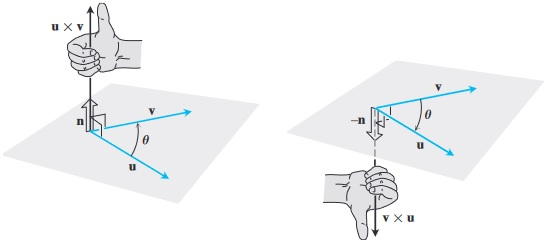
\includegraphics[scale=0.73]{regla-mano-derecha.jpg}
\caption{Thomas (2010). \textit{Cálculo. Varias Variables}. Pp. 682-683.}
\end{figure}

\subsection{Propiedades del producto cruz.}

Sean $\vecmat{a}, \ \vecmat{b}, \ \vecmat{w} \in \R^{3}$ y $c, \ d \in \R$. El producto cruz cumple las siguientes propiedades:
\begin{align*}
&1) \ (c\vecmat{a}) \times (d\vecmat{b}) = (cd) (\vecmat{a} \times \vecmat{b}) &
&2) \ \vecmat{a} \times (\vecmat{b} + \vecmat{w}) = \vecmat{a} \times \vecmat{b} + \vecmat{a} \times \vecmat{w} \\
&3) \ \vecmat{a} \times \vecmat{b} = -(\vecmat{b} \times \vecmat{a}) &
&4) \ (\vecmat{a} + \vecmat{b}) \times \vecmat{w} = \vecmat{a} \times \vecmat{w} + \vecmat{b} \times \vecmat{w} \\
&5) \ \vecmat{0} \times \vecmat{a} = \vecmat{0} &
&6) \ \vecmat{a} \times (\vecmat{b} \times \vecmat{w}) = (\vecmat{a} \cdot \vecmat{w})\vecmat{b} - (\vecmat{a} \cdot \vecmat{b}) \vecmat{w}
\end{align*}

Considere los vectores unitarios estándar $\unitvec{e}_{1} = \langle 1, \ 0, \ 0 \rangle$, $\unitvec{e}_{2} = \langle 0, \ 1, \ 0 \rangle$ y $\unitvec{e}_{3} = \langle 0, \ 0, \ 1 \rangle$.

\newpage

\begin{figure}[hbt!]
\centering

\begin{tikzpicture}
% Líneas de ayuda.
%\draw[color = lightgray] (0, 0) grid (11, 5);

% Ejes de coordenadas.
\draw[-latex, line width = 0.3mm] (5, 2) -- (2.56, 0.56) node[above left] {$x$};
\draw[-latex, line width = 0.3mm] (5, 2) -- (7.3, 0.7) node[above right] {$y$};
\draw[-latex, line width = 0.3mm] (5, 2) node[below] {$0$} -- (5, 4.5) node[left] {$z$};

% Vectores.
\draw[-stealth, line width = 0.6mm, color = red!75] (5, 2) -- node[above left] {$\unitvec{e}_{1}$} (4, 1.4) node[below, color = black] {$1$};
\draw[-stealth, line width = 0.6mm, color = red!75] (5, 2) -- node[above right] {$\unitvec{e}_{2}$} (5.98, 1.46) node[below, color = black] {$1$};
\draw[-stealth, line width = 0.6mm, color = red!75] (5, 2) -- (5, 3) node[right] {$\unitvec{e}_{3}$} node[left, color = black] {$1$};
\end{tikzpicture}

\end{figure}

Mediante la propiedad 3) obtenemos las siguientes igualdades:
\begin{align*}
  \unitvec{e}_{1} \times \unitvec{e}_{2} = -(\unitvec{e}_{2} \times \unitvec{e}_{1}) = \unitvec{e}_{3}, \qquad
  \unitvec{e}_{2} \times \unitvec{e}_{3} = -(\unitvec{e}_{3} \times \unitvec{e}_{2}) = \unitvec{e}_{1}, \qquad
  \unitvec{e}_{3} \times \unitvec{e}_{1} = -(\unitvec{e}_{1} \times \unitvec{e}_{3}) = \unitvec{e}_{2}
\end{align*}
Además:
\[
  \unitvec{e}_{1} \times \unitvec{e}_{1} = \unitvec{e}_{2} \times \unitvec{e}_{2}
                                         = \unitvec{e}_{3} \times \unitvec{e}_{3}
                                         = \vecmat{0}
\]
Si dos vectores \textbf{son iguales}, quiere decir que son \textbf{paralelos}. Por lo tanto, su producto cruz debe ser el vector $\vecmat{0}$.

\subsection{Producto cruz a partir de los componentes.}

Las propiedades del producto cruz permiten obtener una fórmula de ella que depende solo de los componentes de los vectores que la originan.

Sean $\vecmat{a} = a_{1} \unitvec{e}_{1} + a_{2} \unitvec{e}_{2} + a_{3} \unitvec{e}_{3}$ y $\vecmat{b} = b_{1} \unitvec{e}_{1} + b_{2} \unitvec{e}_{2} + b_{3} \unitvec{e}_{3}$. Mediante esta representación, se puede expresar el producto cruz entre ambos vectores como:
\[
  \vecmat{a} \times \vecmat{b} = \vecmat{a} \times
                                 (b_{1} \unitvec{e}_{1} + b_{2} \unitvec{e}_{2} + b_{3} \unitvec{e}_{3})
\]
Por la propiedad 2, esta igualdad es lo mismo que:
\[
  \vecmat{a} \times \vecmat{b} = (\vecmat{a} \times b_{1} \unitvec{e}_{1}) + (\vecmat{a} \times b_{2} \unitvec{e}_{2})
                                 + (\vecmat{a} \times b_{3} \unitvec{e}_{3})
\]
En cada producto cruz del lado derecho se puede aplicar la propiedad 4.
\begin{align*}
  \vecmat{a} \times \vecmat{b} = &(a_{1} \unitvec{e}_{1} \times b_{1} \unitvec{e}_{1}) + (a_{2} \unitvec{e}_{2} \times b_{1} \unitvec{e}_{1}) +
                                 (a_{3} \unitvec{e}_{3} \times b_{1} \unitvec{e}_{1}) + (a_{1} \unitvec{e}_{1} \times b_{2} \unitvec{e}_{2}) +
                                 (a_{2} \unitvec{e}_{2} \times b_{2} \unitvec{e}_{2}) + \\
                                 &(a_{3} \unitvec{e}_{3} \times b_{2} \unitvec{e}_{2}) + (a_{1} \unitvec{e}_{1} \times b_{3} \unitvec{e}_{3}) +
                                 (a_{2} \unitvec{e}_{2} \times b_{3} \unitvec{e}_{3}) + (a_{3} \unitvec{e}_{3} \times b_{3} \unitvec{e}_{3})
\end{align*}
Luego, se puede usar la propiedad 1 en los paréntesis del lado derecho.
\begin{align*}
  \vecmat{a} \times \vecmat{b} = &(a_{1}b_{1}) (\unitvec{e}_{1} \times \unitvec{e}_{1}) + (a_{2}b_{1}) (\unitvec{e}_{2} \times \unitvec{e}_{1}) +
                                 (a_{3}b_{1}) (\unitvec{e}_{3} \times \unitvec{e}_{1}) + (a_{1}b_{2}) (\unitvec{e}_{1} \times \unitvec{e}_{2}) + \\
                                 &(a_{2}b_{2}) (\unitvec{e}_{2} \times \unitvec{e}_{2}) + (a_{3}b_{2}) (\unitvec{e}_{3} \times \unitvec{e}_{2}) +
                                 (a_{1}b_{3}) (\unitvec{e}_{1} \times \unitvec{e}_{3}) + (a_{2}b_{3}) (\unitvec{e}_{2} \times \unitvec{e}_{3}) + \\
                                 &(a_{3}b_{3}) (\unitvec{e}_{3} \times \unitvec{e}_{3})
\end{align*}
Es posible realizar cancelaciones con los $\unitvec{e}_{i} \times \unitvec{e}_{i} = \vecmat{0}$.
\begin{align*}
  \vecmat{a} \times \vecmat{b} = &(a_{2}b_{1}) (\unitvec{e}_{2} \times \unitvec{e}_{1}) + (a_{3}b_{1}) (\unitvec{e}_{3} \times \unitvec{e}_{1}) +
                                 (a_{1}b_{2}) (\unitvec{e}_{1} \times \unitvec{e}_{2}) + (a_{3}b_{2}) (\unitvec{e}_{3} \times \unitvec{e}_{2}) +\\
                                 &(a_{1}b_{3}) (\unitvec{e}_{1} \times \unitvec{e}_{3}) + (a_{2}b_{3}) (\unitvec{e}_{2} \times \unitvec{e}_{3})
\end{align*}
El lado derecho también se puede expresar como:
\begin{align*}
  \vecmat{a} \times \vecmat{b} = &-[(a_{2}b_{1}) \cdot -(\unitvec{e}_{2} \times \unitvec{e}_{1})]
                                 + (a_{3}b_{1}) (\unitvec{e}_{3} \times \unitvec{e}_{1})
                                 + (a_{1}b_{2}) (\unitvec{e}_{1} \times \unitvec{e}_{2}) + \\
                                 &-[(a_{3}b_{2}) \cdot -(\unitvec{e}_{3} \times \unitvec{e}_{2})] +
                                 -[(a_{1}b_{3}) \cdot -(\unitvec{e}_{1} \times \unitvec{e}_{3})]
                                 + (a_{2}b_{3}) (\unitvec{e}_{2} \times \unitvec{e}_{3})
\end{align*}
En la sección 2.2 vimos identidades tales como $\unitvec{e}_{1} \times \unitvec{e}_{2} = -(\unitvec{e}_{2} \times \unitvec{e}_{1}) = \unitvec{e}_{3}$. Al aplicarlas en la ecuación de arriba se obtiene lo siguiente:
\begin{align*}
  \vecmat{a} \times \vecmat{b} = &- (a_{2}b_{1}) \unitvec{e}_{3} + (a_{3}b_{1}) \unitvec{e}_{2} + (a_{1}b_{2}) \unitvec{e}_{3}
                                 - (a_{3}b_{2}) \unitvec{e}_{1} - (a_{1}b_{3}) \unitvec{e}_{2} + (a_{2}b_{3}) \unitvec{e}_{1}
\end{align*}
Finalmente, usando la propiedad 2 podemos factorizar términos comunes del lado derecho.
\[
  \vecmat{a} \times \vecmat{b} = (a_{2}b_{3} - a_{3}b_{2}) \unitvec{e}_{1} - (a_{1}b_{3} - a_{3}b_{1}) \unitvec{e}_{2}
                                 + (a_{1}b_{2} - a_{2}b_{1}) \unitvec{e}_{3}
\]
Esta es la fórmula del producto cruz entre $\vecmat{a}$ y $\vecmat{b}$ usando vectores unitarios estándar. Debido a que su lado derecho se asemeja a la expresión del determinante de tres vectores, también se suele escribir como:
\[
\vecmat{a} \times \vecmat{b} =
\begin{vmatrix}
\unitvec{e}_{1} & \unitvec{e}_{2} & \unitvec{e}_{3} \\
a_{1} & a_{2} & a_{3} \\
b_{1} & b_{2} & b_{3}
\end{vmatrix} =
\unitvec{e}_{1} \cdot
\begin{vmatrix}
a_{2} & a_{3} \\
b_{2} & b_{3}
\end{vmatrix}
- \unitvec{e}_{2} \cdot
\begin{vmatrix}
a_{1} & a_{3} \\
b_{1} & b_{3}
\end{vmatrix}
+ \unitvec{e}_{3} \cdot
\begin{vmatrix}
a_{1} & a_{2} \\
b_{1} & b_{2}
\end{vmatrix}
\]
La expresión de arriba es solo \textbf{simbólica}, ya que el determinante es un escalar y no un vector, como sí lo es el producto cruz.

Por otra parte, se puede expresar al producto cruz en forma componente como:
\[
  \vecmat{a} \times \vecmat{b} = \langle
                                   a_{2}b_{3} - a_{3}b_{2}, \ - (a_{1}b_{3} - a_{3}b_{1}), \ a_{1}b_{2} - a_{2}b_{1}
                                 \rangle
\]

\subsection{Triple producto escalar.}

El producto punto entre un vector y el producto cruz de dos vectores recibe el nombre de \textbf{triple producto escalar}.
\[
  \vecmat{c} \cdot (\vecmat{a} \times \vecmat{b}) = ||\vecmat{c}|| \cdot ||\vecmat{a} \times \vecmat{b}|| \cdot \cos(\theta)
\]
Al expandir el lado izquierdo mediante la definicion algebraica del producto punto, se obtiene lo siguiente:
\[
  \vecmat{c} \cdot (\vecmat{a} \times \vecmat{b}) = (a_{2}b_{3} - a_{3}b_{2})c_{1} - (a_{1}b_{3} - a_{3}b_{1})c_{2} 
                                                    + (a_{1}b_{2} - a_{2}b_{1})c_{3}
\]
El lado derecho corresponde al determinante de $\vecmat{a}, \ \vecmat{b}$ y $\vecmat{c}$ expandido por su tercera fila.
\[
\vecmat{c} \cdot (\vecmat{a} \times \vecmat{b}) =
\begin{vmatrix}
a_{1} & a_{2} & a_{3} \\
b_{1} & b_{2} & b_{3} \\
c_{1} & c_{2} & c_{3}
\end{vmatrix} =
\det(\vecmat{a}, \ \vecmat{b}, \ \vecmat{c})
\]
A continuación veremos que el valor absoluto del triple producto escalar y, por consiguiente, del determinante de sus tres vectores es igual al \textbf{volumen de un paralelelpipedo}.

\subsubsection{Volumen de un paralelepipedo.}

Considere el siguiente paralelepipedo formado por $\vecmat{a}, \ \vecmat{b}, \ \vecmat{c} \in \R^{3}$.

\begin{figure}[hbt!]
\centering

\begin{tikzpicture}
% Líneas de ayuda.
%\draw[color = lightgray] (0, 0) grid (12, 5);

% Área y altura del paralelepipedo.
\draw[color = gray!50, fill = gray!50]  (5, 1) -- (6.5, 1.7) -- (3.5, 1.7) -- (2, 1);
\draw[style = dashed, line width = 0.2mm] (3, 3.2) -- node[right, font = \small] {$h$} (3, 1.2);
\draw (3, 1.45) -- (3.3, 1.45) -- (3.3, 1.2);
\node at (4.5, 1.4) {$A_{\text{base}}$};


% Lados del paralelepipedo.
\draw[line width = 0.3mm] (6, 3.2) -- (7.5, 3.9) -- (4.7, 3.9) -- (3, 3.2) -- (6, 3.2) -- (5, 1) -- (6.5, 1.7) -- (7.5, 3.9);
\draw[style = dashed, line width = 0.3mm] (4.7, 3.9) -- (3.5, 1.7) -- (6.5, 1.7);

% Vectores.
\draw[-stealth, line width = 0.6mm] (2, 1) -- node[below] {$\vecmat{a}$} (5, 1);
\draw[-stealth, line width = 0.6mm] (2, 1) -- node[above] {$\vecmat{b}$} (3.5, 1.7);
\draw[-stealth, line width = 0.6mm] (2, 1) -- (3, 3.2) node[below right] {$\vecmat{c}$};
\end{tikzpicture}

\end{figure}

El volumen del paralelepipedo es el producto entre el área de su base y su altura.
\[
  V_{p} = A_{\text{base}} \cdot h
\]
La base del paralelepipedo es un paralelogramo\footnote{Así como también lo son el resto de sus caras.} que, en este caso, está formado por $\vecmat{a}$ y $\vecmat{b}$. A partir de lo estudiado en la sección 2.1, podemos decir que el área de esta superficie es:
\[
  A_{\text{base}} = ||\vecmat{a} \times \vecmat{b}||
\]
En cuanto a la altura $h$ del paralelepipedo, como es perpendicular a su base, podemos usar la magnitud de un vector unitario normal\footnote{Es lo mismo que ``perpendicular'' u ``ortogonal''.} al plano $\vecmat{n}$ escalado por el componente $c_{3}$ de $\vecmat{c}$.

\begin{figure}[hbt!]
\centering

\begin{tikzpicture}
% Líneas de ayuda.
%\draw[color = lightgray] (0, 0) grid (12, 5);

% Área y altura del paralelepipedo.
\draw[color = gray!50, fill = gray!50]  (5, 1) -- (6.5, 1.7) -- (3.5, 1.7) -- (2, 1);
\draw[style = dashed, line width = 0.2mm] (3, 3.2) -- node[right, font = \small] {$h$} (3, 1.2);
\draw[style = dashed] (3, 3.2) -- (2, 3.2);
\draw (3, 1.45) -- (3.3, 1.45) -- (3.3, 1.2);
\node at (4.5, 1.4) {$A_{\text{base}}$};
\draw (2, 2.9) -- (2.3, 2.9) -- (2.3, 3.2);
\node at (2.2, 2) {$\theta$};


% Lados del paralelepipedo.
\draw[line width = 0.3mm] (6, 3.2) -- (7.5, 3.9) -- (4.7, 3.9) -- (3, 3.2) -- (6, 3.2) -- (5, 1) -- (6.5, 1.7) -- (7.5, 3.9);
\draw[style = dashed, line width = 0.3mm] (4.7, 3.9) -- (3.5, 1.7) -- (6.5, 1.7);

% Vectores.
\draw[-stealth, line width = 0.6mm] (2, 1) -- node[below] {$\vecmat{a}$} (5, 1);
\draw[-stealth, line width = 0.6mm] (2, 1) -- node[above] {$\vecmat{b}$} (3.5, 1.7);
\draw[-stealth, line width = 0.6mm] (2, 1) -- (3, 3.2) node[below right] {$\vecmat{c}$};
\draw[-stealth, line width = 0.6mm, color = red!80] (2, 1) -- (2, 3.2) node[left] {$c_{3} \vecmat{n}$};
\end{tikzpicture}

\end{figure}

En la imagen de arriba se puede ver que $h = ||c_{3}\vecmat{n}||$. Por lo tanto,
\[
  \cos(\theta) = \frac{||c_{3}\vecmat{n}||}{||\vecmat{c}||}
               \Longrightarrow ||c_{3}\vecmat{n}|| = ||\vecmat{c}|| \cdot \cos(\theta)
\]
Así, el volumen del paralelepipedo se puede calcular como:
\[
  V_{p} = | \ ||\vecmat{a} \times \vecmat{b}|| \cdot ||\vecmat{c}|| \cdot \cos(\theta) \ |
        = |\vecmat{c} \cdot (\vecmat{a} \times \vecmat{b})|
        = |\det(\vecmat{a}, \ \vecmat{b}, \ \vecmat{c})|
\]
Se usa el valor absoluto para calcular $V_{p}$ porque el $\cos(\theta) < 0$ para $\frac{\pi}{2} < \theta < \frac{3\pi}{2}$.

\textbf{Ejercicio 1.} Sean $P_{1}, \ P_{2}$ y $P_{3}$ tres puntos de un plano en $\R^{3}$. Evalúe cuál debe ser la condición para que otro punto $P_{4}$ pueda ser miembro de aquella superficie.

\textbf{Solución.} Comencemos definiendo los siguientes dos vectores usando los tres primeros puntos.
\[
  \overvec{P_{1}P_{2}} \qquad \text{y} \qquad \overvec{P_{1}P_{3}}
\]
Luego, busquemos otro vector $\vecmat{v}$ ortogonal al plano mediante el producto cruz entre los dos definidos arriba.
\[
  \vecmat{v} = \overvec{P_{1}P_{2}} \times \overvec{P_{1}P_{3}}
\]
Si $P_{4}$ está en el plano, entonces al formar el vector $\overvec{P_{1}P_{4}}$ debe cumplirse que:
\[
  \overvec{P_{1}P_{4}} \cdot \vecmat{v} = 0
\]
Al reemplazar a $\vecmat{v}$ por $\overvec{P_{1}P_{2}} \times \overvec{P_{1}P_{3}}$ se puede observar lo siguiente:
\begin{align*}
  \overvec{P_{1}P_{4}} \cdot \left(\overvec{P_{1}P_{2}} \times \overvec{P_{1}P_{3}}\right) &= 0 \\
     \det\left(\overvec{P_{1}P_{2}}, \ \overvec{P_{1}P_{3}}, \ \overvec{P_{1}P_{4}}\right) &= 0
\end{align*}
Este resultado indica que, para que $P_{4}$ esté en el plano, su vector creado a partir de $P_{1}$ debe formar un paralelepipedo \textbf{sin volumen}. Así, $\overvec{P_{1}P_{4}}$ será \textbf{coplanar} al igual que $\overvec{P_{1}P_{2}}$ y $\overvec{P_{1}P_{3}}$, lo que puede verificarse cuando el determinante de los tres vectores es igual a cero.

\end{document}
